\documentclass[unknownkeysallowed,final]{beamer}
\usetheme{RJH} %RJH}
\usepackage[orientation=landscape,size=a2,scale=1.4,debug]{beamerposter}
\usepackage[absolute,overlay]{textpos}
\setlength{\TPHorizModule}{1cm}
\setlength{\TPVertModule}{1cm}

\usepackage{amsmath,amsthm, amssymb, latexsym}
\usepackage{multirow}
\usepackage{rotating}

\usepackage{array,booktabs,tabularx}
\newcolumntype{Z}{>{\centering\arraybackslash}X} % centered tabularx columns
\newcommand{\pphantom}{\textcolor{ta3aluminium}} % phantom introduces a vertical space in p formatted table columns??!!
\newcommand{\vectornorm}[1]{\left|\left|#1\right|\right|}

% Poster size can be: 36" wide by 44" tall

\title{\normalsize{Real-Time Activity Classification by Matched Filtering using Body-Worn Accelerometers}}
\author{\small{Craig~Euler craig.euler@gmail.com, C.T.~Lin ct.lin@csun.edu,\\Bryan~Juarez bryan.juarez.974@my.csun.edu, Melissa~Flores melissa.flores.455@my.csun.edu\\College of Engineering and Computer Science\\California State University, Northridge}}

\footer{}
\date{}

\begin{document}
\tiny{}
\begin{frame}{} 

%%
%% Text block
%%
\begin{textblock}{19.5}(1, 7)

\begin{block}{\small{Introduction}}
Various methods for activity classification using body-worn sensors exist.
Custom Decision Tree, Automatically Generated Decision Tree, and Artificial Neural Networks \cite{parkka_ermes_korpipaa_mantyjarvi_peltola_korhonen_2006} have been explored as well as other frequency based classification methods \cite{sharma_purwar_lee_lee_chung_2008}.
The use of the matched-filter method for classification has been studied in the past \cite{giannakis_tsatsanis_1990} and we seek to adopt this method for our use to identify an individual's activity for the purpose of real-time processing on a low-powered micro-controller.
The methods used for our algorithms are designed for computational efficiency to accommodate the resource limitations of a microcontroller. In this paper, we use the MSP432 microcontroller for our timing results.

The algorithms described in this paper are used in two main modules: The activity classification module for real-time processing and the training module to train the device to identify the user's activity.

The training module does not need to be performed in real time.
This algorithm is the most demanding on computational resources and is only executed when training or re-training the unit to identify the user's activity, which means that this can be performed on an external device such as a smart phone or tablet.
The purpose of the training module is to create the reference signals to be used on the microcontroller for the real-time activity classification processing.

The real-time activity classification module is intended to be performed on a low-powered microcontroller.
This module reads in the references stored on the unit to be used as templates that the matched-filter will use for determining the individual's activity.
Both of these modules use the same principles and hence the same algorithm kernels.
\end{block}

%%
%% Activity Classification Method
%%
\begin{block}{\small{Activity Classification Method}}

The matched-filter method is commonly used for extracting a signal out of noisy data.
We use this method for identifying a user's activity from data generated by body-worn accelerometers.
Because the matched-filter method requires use of an existing reference template to identify the desired signal, we must develop our template from a training set.
We will discuss how we develop our set of templates for use in our matched-filter in section \ref{sec:training}.

The matched-filter is based on the cross correlation of the data $\textbf{y} = \{y\}_{k=0}^{N-1}$ with the reference signal $\textbf{x} = \{x\}_{k=0}^{M-1}$.
The cross correlation of $\textbf{x}$ with $\textbf{y}$ is defined as:
%
\begin{equation} \label{eq:cross_correlation}
(\textbf{x} \star \textbf{y}) := \left \{\sum_{i=0}^{M-1}x_{i} y_{i+k} \right \}_{k=0}^{N-M-1}
\end{equation}
%
which is simply a moving dot product.
We can then normalize \eqref{eq:cross_correlation} by the following:
%
\begin{equation} \label{eq:norm_cross_correlation}
\widehat{(\textbf{x} \star \textbf{y})}_k := \frac{(\textbf{x} \star \textbf{y})_k}{||\textbf{x}|| \ || \widetilde{\textbf{y}}_k || }, \quad k = 0,1,...,N-M-1
\end{equation}
%
where $|| \cdot ||$ is the usual $\ell_2$ norm and $\widetilde{\textbf{y}}_k = \{y_p\}_{p=k}^{M+k-1}$.
\eqref{eq:norm_cross_correlation} is now bounded by $[-1,1]$ and has any bias toward high energy removed.
We improve our computational efficiency by applying the convolution theorem to \eqref{eq:cross_correlation} and replacing it with:
%
\begin{equation} \label{eq:conv_theorem}
(\textbf{x} \star \textbf{y}) := FFT^{-1}(FFT(\textbf{x}') FFT(\textbf{y})^*)
\end{equation}
%
where $\textbf{x}'$ is $\textbf{x}$ that has been zero padded to the length of $\textbf{y}$ with the added restriction that the length of $\textbf{x}$ is no more than the length of $\textbf{y}$ and $FFT$ is the Fast Fourier Transform algorithm.
We are most interested where our reference $\textbf{x}$ best matches our data $\textbf{y}$.
We use the resulting max correlation to define our metric for  our matched-filter output as:
%
\begin{equation} \label{eq:matched_filter}
MF_{\textbf{x}}(\textbf{y}) := \underset{k \in [0, M-N)}{max} \left \{\widehat{(\textbf{x} \star \textbf{y})}_k \right \}
\end{equation}
%
If \eqref{eq:matched_filter} passes a set threshold, then the corresponding signal $\textbf{y}$ is classified as a match to the reference $\textbf{x}$.

Applying the convolution theorem to $\eqref{eq:conv_theorem}$ changes the computational complexity or the cross correlation from $\mathcal{O}(n^2)$ to $\mathcal{O}(n log_2n)$.
Despite this reduction in processing cost, the FFTs are still an expensive algorithm for real-time processing on limited hardware resources.
Sections \ref{sec:dim_red} and \ref{sec:decimation} will go into methods that will help reduce the computational burden of the matched-filter.
\end{block}
\end{textblock}

\begin{textblock}{18}(21.8,4)

\begin{block}{\small{Dimensionality Reduction}}





















Classification methods that make use of multi-dimensional feature spaces have increased in popularity and many methods exist \cite{survey_multi_view_machine_learning}.
We manage to reduce our computational resources and remove our dependence on sensor orientation at the same time through a process of dimensionality reduction with principal component analysis (PCA) \cite{bishop_2006}.
Similar to other methods that apply subspace projections \cite{low_rank_subspace}, we seek to analyze our data in a lower dimensional subspace by a projection onto the two-dimension plane that best represents our data.
We assume that over a short period of time, a user's limb movement is constrained mostly to a two-dimensional plane.
By identifying this plane of motion, we then project the acceleration data onto this plane and re-define our new axis accordingly.
%
If we let $\textbf{a} = \{a_i\}_{i=0}^{N}$ represent our demeaned acceleration data (where each $a_i$ is represented as a column) over a specified time window in three dimensions, then the covariance matrix of our acceleration data is represented by the real-symmetric $3 \times 3$ matrix $Q = \textbf{a} \textbf{a}^T$.
The resulting unit length column eigenvectors of $Q$ are $V = (\textbf{v}^1,\textbf{v}^2,\textbf{v}^3)$ with their respective eigenvalues $\lambda^1 \geq \lambda^2 \geq \lambda^3$ of this matrix are orthonormal and point in the directions where the data varies most in descending order for each orthogonal direction.
Here, we use superscripts to identify the axis directions in ascending order to represent the primary, secondary, and tertiary principal axis directions respectively.
%
\begin{equation} \label{eq:project}
   \textbf{a}' := V^T \textbf{a}
\end{equation}
%
We now represent our acceleration data as $\textbf{a}'$ after projecting our acceleration data $\textbf{a}$ onto our rotated axis $V$ by \eqref{eq:project}. If the data is mostly dominate in the two primary dimensions, i.e. $\lambda^3 << \lambda^2$, then it is safe to assume that
%
\begin{equation} \label{eq:magnitude}
||(a_x,a_y,a_z)||^2 = ||(a'^1,a'^2,a'^3)||^2 \sim = (a'^1)^2 + (a'^2)^2
\end{equation}
$ \forall a \in \textbf{a}. $ \\
%
Where equality comes from the orthonormality of $V$.
By now, we have preserved as much information that is contained in our acceleration data as possible in the process of reducing our dimensions from three to two.

In this paper, we compute the matched-filter output for two dimensions by generalizing \eqref{eq:matched_filter} by augmenting our reference and signal with both dimensions appropriately for normalization and adding together the cross correlations as:
%
\begin{equation} \label{eq:cross_correlation_2}
\widehat{(\textbf{x}^{1,2} \star \textbf{y}^{1,2})}_k := \frac{(\textbf{x}^1 \star \textbf{y}^1)_k + (\textbf{x}^2 \star \textbf{y}^2)_k}{||[ \textbf{x}^1, \textbf{x}^2 ]|| \ || [ \widetilde{\textbf{y}}_k^1, \widetilde{\textbf{y}}_k^2 ] || },
\end{equation}
%
for $ k = 0,1,...,N-M-1 $. \\
%
\begin{equation} \label{eq:matched_filter_2}
MF_{\textbf{x}}^2(\textbf{y}) := \underset{k \in [0, M-N)}{max} \left \{\widehat{(\textbf{x}^{1,2} \star \textbf{y}^{1,2})}_k \right \}
\end{equation}
%
This works because both dimensions are always in phase with each other for any given activity and therefore the match will happen in sync. Here, the superscripts $1$ and $2$ represent the primary and secondary principal components of our data respectively.
%











\end{block}

\begin{block}{\small{Decimation}}
Decimation is the first step applied to our data before any additional processing takes place.
Decimation is a process of reducing the sampling rate of the signal by filtering to mitigate any possible distortion effects due to aliasing followed by downsampling.
Because real-time performance is important, we decimate our signal for the purpose of improving our throughput.

For a decimation value of $D$, we define our triangle filter with the following weights:
%
\begin{equation} \label{eq:triangle_filter_weights}
w_k^D :=
\begin{cases}
  \frac{D+k}{D^2}, & \text{if }\ -D < k \leq 0 \\
  \frac{D-k}{D^2}, & \text{if } 0 < k < D \\
  0, & \text{otherwise}
\end{cases}
\end{equation}
%
and convolve it with our data to get
%
\begin{equation} \label{eq:convolve}
s'_k := \sum_{i=0}^{N} s_i w_{k-i}
\end{equation}
%
followed by a downsample
%
\begin{equation} \label{eq:downsample}
s''_k := s'_{(k+1)D-1}, \quad k = 0, 1, 2, ..., N/D.
\end{equation}
%
The processing cost is reduced by only processing points in \eqref{eq:convolve} that we keep in \eqref{eq:downsample}.
\end{block}


\end{textblock}

%%
%% Text block
%%
\begin{textblock}{17.3}(41,4)
\begin{block}{\small{Training the Module}}















We are able to identify an individual's activity by matching the signal to a reference template.
For our application, we develop a reference template for our matched-filter directly from the person's motion signature.
We do this by having the individual perform the specific activity over a specified amount of time and select the sub-interval of time that we find best represents the user's motion signature.
For a given activity, we attempt to find the representative periodic signal $\textbf{s}$ of our individual's activity to be our template for our matched-filter.

If $\textbf{t} = \{t_k\}_{k=0}^{N_t}$ is our training set over $N_t$ data points, we define a collection of subsets $X$ of $\textbf{t}$:
%
\begin{equation} \label{eq:X_subsets_of_training_eq}
X := \left \{ \{t_k\}_{k=p}^{p+M-1} | p=mI \right \}
\end{equation}
%
and $Y$ of $\textbf{t}$:
%
\begin{equation} \label{eq:Y_subsets_of_training_eq}
Y := \left \{ \{t_k\}_{k=p}^{p+N-1} | p=nI \right \}
\end{equation}
%
where $M \leq N$, $I$ is a positive, fixed integer, and $(m,n) \in \mathbb{Z}^2$ where $(m,n)$ vary such that $0 \leq (m,n)I$ and $(m,n)I + (M,N) - 1 \leq N_t$. Then we can determine the representative signal $\textbf{s} \in X$ for our activity that satisfies the condition:
%
\begin{equation} \label{eq:s_condition}
\sum_{y \in Y}MF^2_{\textbf{s}}(\textbf{y}) \geq \sum_{y \in Y}MF^2_{\textbf{x}}(\textbf{y}), \quad \forall \textbf{x} \in X
\end{equation}

We chose this method for its simplicity and robustness against outliers in our training set. We anticipate that the user will have idle motion at the start and end of their training duration when they activate the training mode and with possible disruptions during the process.










































\begin{center}
% 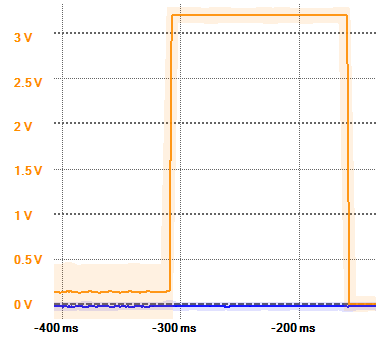
\includegraphics[scale=.75]{reference_pulse_32Hz_4sec_8downsample_2.png}
\end{center}
\end{block}

\begin{block}{\small{References}}
\bibliographystyle{plain}
\bibliography{reference}
\end{block}
\end{textblock}

\end{frame}
\end{document}
